\documentclass[final]{article}

\usepackage[final,main]{APS360}
\usepackage[utf8]{inputenc}
\usepackage[T1]{fontenc}
\usepackage{hyperref}
\hypersetup{hidelinks}
\usepackage{url}
\usepackage{booktabs}
\usepackage{amsfonts}
\usepackage{amsmath}
\usepackage{nicefrac}
\usepackage{microtype}
\usepackage{xcolor}
\usepackage{graphicx}
\usepackage{subcaption}
\usepackage{tikz}
\usetikzlibrary{arrows.meta,positioning}
\usepackage{natbib}

\title{Robust Cross-Day Hand-Gesture Recognition from\\
Wrist Surface Electromyography Using a 1D~CNN}

\author{%
  Grace MacLeod \\
  \mbox{} \\
  \url{https://github.com/gracemacleodd/APS360-EMG-Gesture-Recognition}
}

\begin{document}

\maketitle
\vspace{-0.5in}

% ======================================================================
%  SECTION 1 — Brief Project Description (5 pts)
% ======================================================================
\section{Brief Project Description}

Surface electromyography (sEMG) records the electrical activity of contracting muscles and is a leading modality for wearable human--computer interfaces, prosthetic control, and rehabilitation. The dominant obstacle to deployment is \emph{cross-day degradation}: a model trained on one recording day loses accuracy on a later day as electrode placement, skin impedance, and muscle state shift between sessions~\citep{kaifosh2025}. This project asks whether a learned-feature 1D convolutional neural network (CNN) generalizes across recording days better than a traditional feature-engineered support-vector machine (SVM), on 16 static hand/finger gestures from 12-channel wrist sEMG. Deep learning is a natural fit: the raw multichannel signal contains temporal and inter-channel structure that hand-crafted features may discard, so a CNN can learn task-specific, potentially session-invariant filters directly from data.

\begin{figure}[!h]
  \centering
  \resizebox{0.85\textwidth}{!}{%
  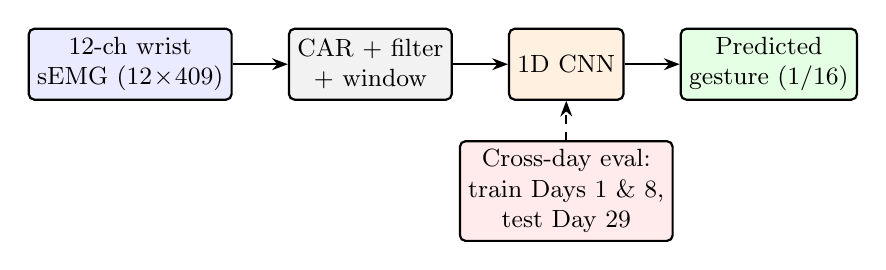
\begin{tikzpicture}[
      node distance=4mm,
      box/.style={rectangle, rounded corners=2pt, draw=black, thick,
                  align=center, inner sep=3pt, minimum height=9mm, font=\small},
      arr/.style={-{Stealth[length=2mm]}, thick}
    ]
    \node[box,fill=blue!8] (in) {12-ch wrist\\sEMG ($12\!\times\!409$)};
    \node[box,right=7mm of in,fill=gray!10] (proc) {CAR + filter\\+ window};
    \node[box,right=7mm of proc,fill=orange!12] (model) {1D CNN};
    \node[box,right=7mm of model,fill=green!10] (out) {Predicted\\gesture (1/16)};
    \node[box,below=5mm of model,fill=red!8,font=\small] (eval) {Cross-day eval:\\train Days 1 \& 8,\\test Day 29};
    \draw[arr] (in) -- (proc);
    \draw[arr] (proc) -- (model);
    \draw[arr] (model) -- (out);
    \draw[arr,dashed] (eval) -- (model);
  \end{tikzpicture}%
  }
  \caption{CNN pipeline: wrist sEMG windows in, gesture class out. Cross-day trains on Days~1 and~8, tests on Day~29. The SVM baseline (Sec.~2.2) uses extracted features.}
  \label{fig:pipeline}
\end{figure}

% ======================================================================
%  SECTION 2 — Notable Contribution (15 pts)
% ======================================================================
\section{Notable Contribution}

\subsection{Data Processing}

\textbf{Source.}
We use the open-access GRABMyo dataset~\citep{pradhan2022grabmyo,jiang2022grabmyophysionet} (PhysioNet, v1.0.1): 43 participants recorded across three separated days (Days~1, 8, and 29) performing 16 gestures over 7 trials each at 2048\,Hz. We restrict to the 12 wrist sEMG channels (dataset columns 18--23 and 26--31; 0-based Python indices 17--22 and 25--30) and use the first 25 participants as a computational development subset selected before evaluating model performance. The complete 43-participant dataset is publicly available on PhysioNet; the final evaluation will scale to all 43.

\textbf{Cleaning.}
Each channel is common-average referenced (CAR) across the 12 wrist electrodes, then zero-phase band-pass filtered (4th-order Butterworth, 20--450\,Hz via \texttt{sosfiltfilt}), and finally 60\,Hz notch-filtered ($Q\!=\!30$). No trials were excluded; visual inspection of the filtered signals revealed no flat or saturated channels. Figure~\ref{fig:cleaned} shows a raw vs.\ cleaned channel with a 200\,ms analysis window highlighted.

\textbf{Windowing and statistics.}
Filtered signals are segmented into $\sim$200\,ms windows (409 samples, stride 204) at ${\sim}$50\% overlap~\citep{smith2011window}, yielding \textbf{411{,}600} total windows balanced across 16 gestures (25{,}725 per class). Splits are defined at the \emph{trial level before windowing} so overlapping windows never span two splits. The same-day protocol pools Days~1 and~8, splitting by trial: train \{1,2,3,5\} / val \{6\} / test \{4,7\} $\to$ 156{,}800 / 39{,}200 / 78{,}400 windows. Cross-day trains on trials 1--6 of Days~1 and~8, validates on trial~7, and tests on all of Day~29 $\to$ 235{,}200 / 39{,}200 / 137{,}200 windows. Per-channel mean and standard deviation are computed on each protocol's training set only.

\textbf{Unseen-data plan.}
For final testing we plan to evaluate on NinaPro~DB2~\citep{atzori2014ninapro}, an entirely different sEMG dataset not used during development, serving as an external-domain robustness test with an explicit label mapping to the subset of shared gestures.

\textbf{Challenges.}
The full dataset exceeds Colab's RAM when loaded at once; we implemented a two-pass memory-safe reassembly that preallocates the output array and streams one participant shard at a time.

\begin{figure}[!h]
  \centering
  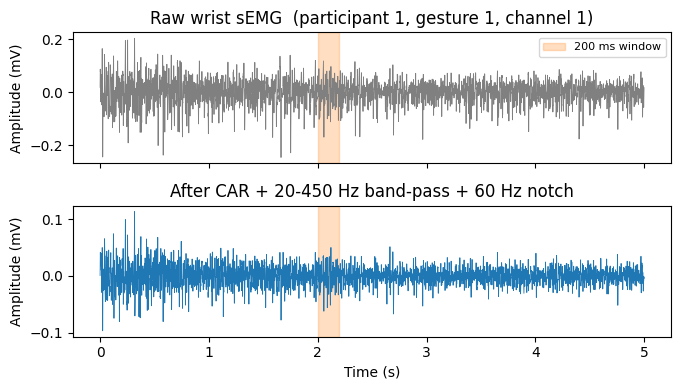
\includegraphics[width=0.70\linewidth]{figs/cleaned_sample.png}
  \caption{Cleaned training sample: raw (top) vs.\ filtered (bottom) wrist sEMG, participant~1, gesture~1, channel~1. Orange band = one 200\,ms window.}
  \label{fig:cleaned}
\end{figure}

\subsection{Baseline Model}

The baseline extracts four Hudgins time-domain features~\citep{hudgins1993strategy}---root-mean-square, mean absolute value, waveform length, and zero crossings (sign-change count, no amplitude threshold)---per channel from each window, giving a 48-dimensional vector. Features are standardized (zero mean, unit variance) using training-set statistics only, then classified by an RBF-kernel SVM with manually selected $C\!=\!10$ and $\gamma\!=\!\text{scale}$. Because kernel-SVM training scales super-linearly, the training set is capped at 12{,}000 windows sampled uniformly at random (seed~0).

\textbf{Quantitative results.}
The SVM achieves 66.5\% same-day and 51.0\% cross-day accuracy (Table~\ref{tab:results})---well above the 6.25\% chance level---with a cross-day drop of 15.5 percentage points.

\textbf{Qualitative results.}
Figure~\ref{fig:cm}a shows the SVM's cross-day confusion matrix. The off-diagonal spread is broad: the worst confusion is true Thumb Extension (TE) predicted as Thumb--Index Finger Extension (TIFE) at 23.7\%, followed by TLFO$\to$IMFE at 18.4\%---errors that may reflect overlapping forearm-muscle activation patterns between gestures.

\textbf{Challenges.}
Capping training at 12{,}000 windows is an acknowledged confound when comparing absolute accuracy with the CNN. We treat each model's within-model cross-day drop as a protocol-level robustness indicator rather than a perfectly controlled domain-shift estimate.

\subsection{Primary Model}

The 1D~CNN (Figure~\ref{fig:arch}) treats each window as a 12-channel, length-409 time series. It stacks three convolutional blocks---each Conv1D (kernel~5, padding~2), batch normalization, ReLU, max-pool by~2---widening channels $12\!\to\!32\!\to\!64\!\to\!128$. Global average pooling collapses the temporal axis, dropout ($p\!=\!0.3$) regularizes, and two FC layers ($128\!\to\!64\!\to\!16$) produce logits. The network has \textbf{63{,}088 trainable parameters}. Training uses Adam (lr $10^{-3}$, weight decay $10^{-4}$), cross-entropy loss, batch size 256, mixed-precision on GPU, \texttt{ReduceLROnPlateau} scheduling, and early stopping (patience~8) on validation macro-F1.

\begin{figure}[!h]
  \centering
  \resizebox{\textwidth}{!}{%
  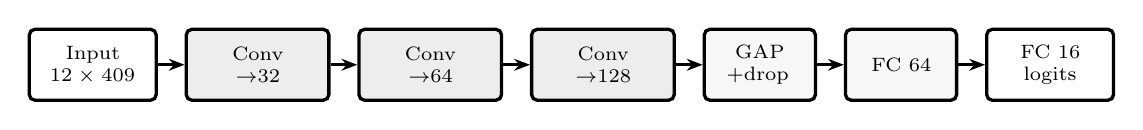
\begin{tikzpicture}[
      node distance=3.4mm,
      io/.style={rectangle, rounded corners=2pt, draw=black, very thick,
                 align=center, inner sep=3pt, minimum height=9mm, font=\scriptsize,
                 text width=14mm},
      conv/.style={rectangle, rounded corners=2pt, draw=black, very thick,
                   fill=black!7, align=center, inner sep=3pt, minimum height=9mm,
                   font=\scriptsize, text width=16mm},
      fc/.style={rectangle, rounded corners=2pt, draw=black, very thick,
                 fill=black!3, align=center, inner sep=3pt, minimum height=9mm,
                 font=\scriptsize, text width=12mm},
      arr/.style={-{Stealth[length=2mm]}, very thick}
    ]
    \node[io] (in) {Input\\$12\times409$};
    \node[conv, right=of in] (c1) {Conv\\$\to$32};
    \node[conv, right=of c1] (c2) {Conv\\$\to$64};
    \node[conv, right=of c2] (c3) {Conv\\$\to$128};
    \node[fc, right=of c3] (gap) {GAP\\+drop};
    \node[fc, right=of gap] (f1) {FC 64};
    \node[io, right=of f1] (out) {FC 16\\logits};
    \draw[arr] (in) -- (c1);
    \draw[arr] (c1) -- (c2);
    \draw[arr] (c2) -- (c3);
    \draw[arr] (c3) -- (gap);
    \draw[arr] (gap) -- (f1);
    \draw[arr] (f1) -- (out);
  \end{tikzpicture}%
  }
  \caption{1D~CNN (63{,}088 params). Each Conv block: Conv1D(5)$\to$BN$\to$ReLU$\to$MaxPool2.}
  \label{fig:arch}
\end{figure}

\textbf{Quantitative results.}
The CNN achieves 85.2\% same-day and 74.1\% cross-day accuracy (Table~\ref{tab:results}), outperforming the SVM in every setting. Its cross-day drop is 11.1 percentage points versus the SVM's 15.5, consistent with learned convolutional features being more robust to the day-to-day domain shift. The comparison does not fully isolate architecture from training-set size (the SVM is capped at 12{,}000 windows), so the within-model drop serves as a protocol-level robustness indicator. All metrics are computed on the pooled test set across participants.

\begin{table}[!h]
  \centering
  \caption{Test accuracy and macro-F1 (25 participants, 16 gestures). 411{,}600 is the total processed dataset; per-protocol test sizes are 78{,}400 (same-day) and 137{,}200 (cross-day). ``Drop'' = same-day $-$ cross-day accuracy.}
  \label{tab:results}
  \small
  \begin{tabular}{lccccc}
    \toprule
     & \multicolumn{2}{c}{Same-day} & \multicolumn{2}{c}{Cross-day} & Cross-day \\
    \cmidrule(lr){2-3}\cmidrule(lr){4-5}
    Model & Acc & F1 & Acc & F1 & drop \\
    \midrule
    RBF-SVM (Hudgins) & 0.665 & 0.665 & 0.510 & 0.508 & 0.155 \\
    1D CNN            & \textbf{0.852} & \textbf{0.852} & \textbf{0.741} & \textbf{0.740} & \textbf{0.111} \\
    \bottomrule
  \end{tabular}
\end{table}

\textbf{Qualitative results.}
Figure~\ref{fig:cm} compares the cross-day confusion matrices (row-normalized, shared 0--100\% colour scale). The CNN's diagonal is darker and its off-diagonal mass more contained. Its top confusions are TLFO$\to$IMFE (19.0\%) and IMFE$\to$TLFO (15.0\%)---a symmetric pair that may reflect similar finger-opposition mechanics---plus LP$\to$HC (14.5\%), where the lateral pinch and hand close may share overlapping grip-muscle activation. The SVM's worst confusion (TE$\to$TIFE, 23.7\%) is both larger and reflects a broader difficulty distinguishing extension gestures. Notably, cross-day validation macro-F1 plateaus near 0.85--0.87 on Days~1 and~8, while held-out Day-29 test macro-F1 is 0.740---directly illustrating the cross-day domain shift.

\begin{figure}[!h]
  \centering
  \begin{subfigure}{0.49\textwidth}
    
\includegraphics[width=\linewidth]{figs/cm_svm_cross_pct.png}
    \caption{SVM, cross-day}
  \end{subfigure}
  \hfill
  \begin{subfigure}{0.49\textwidth}
    
\includegraphics[width=\linewidth]{figs/cm_cnn_cross_pct.png}
    \caption{CNN, cross-day}
  \end{subfigure}
  \caption{Cross-day confusion matrices (row-normalized \%, shared 0--100\% scale). The CNN's errors are more contained along the diagonal.}
  \label{fig:cm}
\end{figure}

\textbf{Challenges and feasibility.}
Validation is drawn from Days~1 and~8 and does not reflect the Day-29 shift; the true cross-day performance is the held-out test accuracy. The cross-day CNN reached the 60-epoch cap without early stopping; whether additional training helps will be examined. Training takes $\sim$5--7 min per CNN on Colab~Pro, so the remaining work is tractable.

\bibliographystyle{plainnat}
\bibliography{references}

\end{document}
